% !TEX TS-program = XeLaTeX
% use the following command:
% all document files must be coded in UTF-8
\documentclass[english]{textolivre}
% build HTML with: make4ht -e build.lua -c textolivre.cfg -x -u article "fn-in,svg,pic-align"


\journalname{Texto Livre}
\thevolume{18}
%\thenumber{1} % old template
\theyear{2025}
\receiveddate{\DTMdisplaydate{2025}{5}{8}{-1}} % YYYY MM DD
\accepteddate{\DTMdisplaydate{2025}{7}{5}{-1}}
\publisheddate{\DTMdisplaydate{2025}{9}{22}{-1}}
\corrauthor{Pedro Jerónimo}
\articledoi{10.1590/1983-3652.2025.59031}
%\articleid{NNNN} % if the article ID is not the last 5 numbers of its DOI, provide it using \articleid{} commmand 
% list of available sesscions in the journal: articles, dossier, reports, essays, reviews, interviews, editorial
\articlesessionname{articles}
\runningauthor{Jerónimo and Torre} 
%\editorname{Leonardo Araújo} % old template
\sectioneditorname{Daniervelin Pereira}
\layouteditorname{Saula Cecília}

\title{Local journalism in the digital age: a systematic review of a decade of research}
\othertitle{Jornalismo local na era digital: revisão sistemática de uma década de pesquisa}
% if there is a third language title, add here:
%\othertitle{Artikelvorlage zur Einreichung beim Texto Livre Journal}

\author[1]{Pedro Jerónimo~\orcid{0000-0003-1900-5031}\thanks{Email: \href{mailto:pj@ubi.pt}{pj@ubi.pt}}}
\author[1]{Luisa Torre~\orcid{0000-0002-5948-106X}\thanks{Email: \href{mailto:luisa.torre@ubi.pt}{luisa.torre@ubi.pt}}}
\affil[1]{University of Beira Interior, Faculty of Arts and Letters, Department of Communication, Philosophy and Politics, LabCom - Communication Laboratory, Covilhã, Portugal.}


\addbibresource{article.bib}
% use biber instead of bibtex
% $ biber article

% used to create dummy text for the template file
\definecolor{dark-gray}{gray}{0.35} % color used to display dummy texts
\usepackage{lipsum}
\SetLipsumParListSurrounders{\colorlet{oldcolor}{.}\color{dark-gray}}{\color{oldcolor}}

% used here only to provide the XeLaTeX and BibTeX logos
\usepackage{hologo}

% if you use multirows in a table, include the multirow package
\usepackage{multirow}

% provides sidewaysfigure environment
\usepackage{rotating}

% CUSTOM EPIGRAPH - BEGIN 
%%% https://tex.stackexchange.com/questions/193178/specific-epigraph-style
\usepackage{epigraph}
\renewcommand\textflush{flushright}
\makeatletter
\newlength\epitextskip
\pretocmd{\@epitext}{\em}{}{}
\apptocmd{\@epitext}{\em}{}{}
\patchcmd{\epigraph}{\@epitext{#1}\\}{\@epitext{#1}\\[\epitextskip]}{}{}
\makeatother
\setlength\epigraphrule{0pt}
\setlength\epitextskip{0.5ex}
\setlength\epigraphwidth{.7\textwidth}
% CUSTOM EPIGRAPH - END

% to use IPA symbols in unicode add
%\usepackage{fontspec}
%\newfontfamily\ipafont{CMU Serif}
%\newcommand{\ipa}[1]{{\ipafont #1}}
% and in the text you may use the \ipa{...} command passing the symbols in unicode

% LANGUAGE - BEGIN
% ARABIC
% for languages that use special fonts, you must provide the typeface that will be used
% \setotherlanguage{arabic}
% \newfontfamily\arabicfont[Script=Arabic]{Amiri}
% \newfontfamily\arabicfontsf[Script=Arabic]{Amiri}
% \newfontfamily\arabicfonttt[Script=Arabic]{Amiri}
%
% in the article, to add arabic text use: \textlang{arabic}{ ... }
%
% RUSSIAN
% for russian text we also need to define fonts with support for Cyrillic script
% \usepackage{fontspec}
% \setotherlanguage{russian}
% \newfontfamily\cyrillicfont{Times New Roman}
% \newfontfamily\cyrillicfontsf{Times New Roman}[Script=Cyrillic]
% \newfontfamily\cyrillicfonttt{Times New Roman}[Script=Cyrillic]
%
% in the text use \begin{russian} ... \end{russian}
% LANGUAGE - END

% EMOJIS - BEGIN
% to use emoticons in your manuscript
% https://stackoverflow.com/questions/190145/how-to-insert-emoticons-in-latex/57076064
% using font Symbola, which has full support
% the font may be downloaded at:
% https://dn-works.com/ufas/
% add to preamble:
% \newfontfamily\Symbola{Symbola}
% in the text use:
% {\Symbola }
% EMOJIS - END

% LABEL REFERENCE TO DESCRIPTIVE LIST - BEGIN
% reference itens in a descriptive list using their labels instead of numbers
% insert the code below in the preambule:
%\makeatletter
%\let\orgdescriptionlabel\descriptionlabel
%\renewcommand*{\descriptionlabel}[1]{%
%  \let\orglabel\label
%  \let\label\@gobble
%  \phantomsection
%  \edef\@currentlabel{#1\unskip}%
%  \let\label\orglabel
%  \orgdescriptionlabel{#1}%
%}
%\makeatother
%
% in your document, use as illustraded here:
%\begin{description}
%  \item[first\label{itm1}] this is only an example;
%  % ...  add more items
%\end{description}
% LABEL REFERENCE TO DESCRIPTIVE LIST - END


% add line numbers for submission
%\usepackage{lineno}
%\linenumbers

\begin{document}
\maketitle

\begin{polyabstract}
\begin{abstract}
This paper summarizes research on digital local journalism conducted between 2013 and 2023. Through a systematic literature review (n=149), six research clusters were identified: journalistic practices, media landscapes, digital transformation, audience engagement, business models, and civic participation. The findings highlight the dual challenges of innovation and sustainability, especially for smaller media outlets in resource-scarce contexts. Local journalism continues to play a key role in community identity, despite threats to its future posed by the spread of news deserts, the dangers of algorithmic biases and funding difficulties. These results also stress the intrinsic connection between technological innovation, business model sustainability, and the fostering of civic participation, all of which are essential to the resilience of local journalism. Research remains concentrated in the Global North, pointing to the need for broader geographical representation. Future studies are suggested regarding the ethical use of Artificial Intelligence, hyperlocal resilience, and mechanisms for building trust.

\keywords{Local journalism\sep Digital journalism\sep News production\sep Local media\sep Systematic review}
\end{abstract}

\begin{portuguese}
\begin{abstract}
Este artigo sintetiza a pesquisa sobre jornalismo local digital realizada entre 2013 e 2023. Mediante uma revisão sistemática da literatura (n=149), foram identificados seis agrupamentos de pesquisa: práticas jornalísticas, panoramas mediáticos, transformação digital, envolvimento da audiência, modelos de negócio e participação cívica. Os resultados enfatizam o duplo desafio da inovação e sustentabilidade, especialmente para os media menores e em contextos de escassez de recursos, enquanto o jornalismo local continua a desempenhar um papel fundamental na identidade das comunidades, apesar de o seu futuro ser ameaçado por desertos de notícias, vieses algorítmicos e déficits de financiamento. Também sublinham a intrínseca ligação entre a inovação tecnológica, a sustentabilidade dos modelos de negócio e o fomento da participação cívica, essenciais para a resiliência do jornalismo local. A pesquisa permanece concentrada no Norte Global, apontando para a necessidade de uma representação geográfica mais ampla. Sugerem-se futuros estudos que abordem o uso ético de Inteligência Artificial, a resiliência hiperlocal e mecanismos de construção de confiança.

\keywords{Jornalismo local\sep Jornalismo digital\sep Produção de notícias\sep Media locais\sep Revisão sistemática}
\end{abstract}
\end{portuguese}
% if there is another abstract, insert it here using the same scheme
\end{polyabstract}

\section{Introduction}
Thirty years after the internet first became central in newsrooms, new challenges are emerging. Social networks and search engines have transformed the way news is distributed, traditional business models have proved increasingly unviable, the proliferation of disinformation has intensified into a significant crisis, and the most recent advances in Artificial Intelligence (AI) have introduced new layers of complexity.

Early research on digital journalism focused mainly on its distribution and product characteristics, followed by studies using an ethnographic approach \cite{jeronimo2015}. Transformations in working conditions were also considered \cite{deuze2009, morais2020}. More recent studies concentrate on themes of technology, platforms, and audiences \cite{steensen2019}, exploring how the ``digital" sphere affects, and is affected by, journalism in society. Digital journalism research is positioned between continuity and change: it analyses the crisis facing the media, journalism’s processes of innovation and adaptation, and the continued blurring of boundaries between journalists and audiences, facts and opinions, and real and fake news \cite{eldridge2019, westlund2023}.

Scholars have employed diverse terminologies to refer to digital journalism, with English- and Latin American-speaking communities preferring ``online journalism" or ``digital journalism" \cite{boczkowski2004, westlund2023, eldridge2019}, while Portuguese- and Spanish-speaking communities mainly use ``cyberjournalism" \cite{bastos2023, jeronimo2015, diaz2003, lopez-garcia2008}. Although terms such as ``online journalism" and ``multimedia journalism" dominated early studies, ``digital journalism" gained prominence after 2010, with the launch of the scientific journal Digital Journalism in 2013 \cite{steensen2019}. Regardless of terminology, these all refer to journalism which is disseminated online, even in the case of local news \cite{jeronimo2015}.

Digital journalism is now considered an ``established discipline". However, some challenges still need to be addressed, including a need for a stronger focus on digital native, or exclusively digital, media outlets, for conducting innovation-oriented research, and for paying greater attention to under-researched topics and areas \cite{salaverria2019} -- local journalism is one such overlooked topic, a gap which this article seeks to address. The close relationship between local media and their audience empowers journalists to develop specific agenda-setting processes, thanks to tighter connections with the publics they aim to inform \cite{correia2019fake}. In this way, local news results from a journalistic practice which is committed to a territory and to the people who are geographically or emotionally connected to it -- communities with which journalists share cultural values and social spaces, and to which they often belong themselves \cite{camponez2002, lopez-garcia2008}. Belonging to  the same communities allows journalists to gain deeper knowledge of the events they cover, but such proximity may result in a lack of independence and distance required by journalistic ethical precepts \cite{jeronimo2015}. These media outlets play a fundamental role in meeting the informational needs of local communities while shaping how community members perceive themselves and their local realities \cite{nielsen2015}.

Journalism has faced changes caused by losing its exclusivity in the production and dissemination of information, which the public is now also able to do \cite{castells2015}. Algorithmic gatekeeping has emerged as a relevant mechanism of news visibility and disinformation dissemination \cite{cardoso2023}. Large technology companies have absorbed most of the advertising revenues that used to sustain the media business, affecting local media especially \cite{costa2014}. Journalists face an increasingly fast-paced working environment, marked by the pursuit of technological innovation, which is altering newsroom tasks and organisation. The integration of automation and AI affects news production, distribution, and reception, including in smaller newsrooms \cite{goncalves2024}. In this changing world, which also impacts the work of local journalists, what themes and challenges emerge from research carried out between 2013 and 2023?

Recent literature reviews on local journalism have focused on hyperlocal media \cite{negreira-rey2021, negreira-rey_amigo2022}, news deserts \cite{rodriguezurra2024}, and the erosion of proximity in local journalism \cite{mota2023}. However, studies on digital journalism at a local scale – or proximity cyberjournalism, as other authors argue \cite{lopez-garcia2008, jeronimo2015} – remain relatively underexplored, particularly in light of the challenges posed by disinformation, social media usage, and the impact of platformisation \cite{poell2020plataformizacao, morais2023}. This article explores changes in local digital journalism, highlighting technological challenges, impacts on democracy, and information dynamics in small communities. This observation relates to the role of local journalistic information in community identity and cohesion. By connecting people in digital and physical spaces through shared social and cultural values, local journalism functions as a ``social glue" that fosters a sense of community \cite{hess2015}.

The period under study (2013–2023) is marked by a rapid process of digitisation and profound changes in media–audience interaction \cite{heiselberg2024}. We aim to investigate whether research interest in the efield has grown over this interval and whether the most relevant journals are devoting space to this topic, in order to understand its relevance within the broader field of digital journalism studies. We also aim to identify the main topics of research and to assess whether research into local digital journalism has evolved towards a greater focus on technology, platforms, and audiences -- as has been observed more broadly in digital journalism research \cite{steensen2019} -- or whether other themes tied to a more local approach have emerged. In addition, we seek to determine which countries are most frequently studied, and evaluate whether some regions remain under-researched and could benefit from future studies, or whether trends of disparate thematic preferences exist within different regions. Through a systematic review of the literature on local digital journalism, we intend to analyse and understand the research conducted over the past ten years in this field. Based on this overview and the identified gaps in the literature, we aim to answer the following questions:

\begin{itemize}
    \item RQ1. What themes and methodologies have been adopted in local digital journalism research in the past decade (2013-2023), and how do they reflect the challenges and transformations in the field?
    \item RQ2. What are the most frequently studied geographical contexts, in which journals is this research published, and how do such  patterns affect the global understanding of local digital journalism?  
\end{itemize}


\section{Material and methods}
This study was conducted as a systematic literature review, with the aim of mapping and analysing research on local digital journalism. The chosen methodology prioritises transparency and replicability, focusing on scientific publications to ensure data quality. The choice of texts published exclusively in English is justified by the prevalence and impact of academic output in this language within international communication databases, which ensures an analysis centred on literature with the widest global reach within the defined period (2013–2023). Data extraction was carried out using the Scopus database, recognised for its breadth in scientific journals, ensuring relevant coverage for the field. Data analysis was carried out in two separate stages: initially, a quantitative approach was used to identify numerical trends (such as the journal and year of publication  and author affiliations), followed by an in-depth qualitative analysis to categorise and discuss the predominant themes and methodologies of these scientific articles. This structure is intended to provide a clear understanding of research trends and gaps.

Data extraction took place between September and October 2024, and inclusion criteria comprised publications focusing on local digital journalism, showing strong correspondence with the selected keywords and categories (``Social Sciences" and ``Arts and Humanities"), falling within the proposed period, and published in English. Exclusion criteria included duplicate results for the selected keywords, non-corresponding topics, and an overly narrow framing when analysing local media, as well as studies not addressing local digital journalism.

A total of 18 keyword combinations were searched, resulting in 1,529 entries. Of these, 692 references were excluded due to duplication or lack of strong correspondence with the keywords, leaving 837 entries. The keyword search included combinations of the terms ``digital", ``online", or ``cyber"; ``local" and ``proximity"; ``journalism", ``journalists", and ``news". Abstracts of the publications were then read and, in some cases, a superficial reading of the full text was also done to support the decision of inclusion or exclusion.

Exclusion criteria included: articles not in English; abstracts unavailable online; articles broadly referring to local journalism or local news without a focus on the digital aspect. Studies focusing on other topics related to local journalism (e.g. public service media or ethnic media) but not centred on the digital dimension of analysis were not included. Research on local news audiences that did not differentiate between digital and offline audiences was excluded. Topics closely related to local journalism (e.g. hyperlocal, citizen journalism, community journalism, ``news deserts"), which discussed digital news organisations or journalists, were included and grouped into thematic clusters. Publications addressing local online journalism alongside traditional/offline local media (comparisons, etc.) were also included in the sample. The systematic application of the exclusion criteria resulted in the removal of 688 publications, one of which lacked an abstract, leaving a final sample of 149 publications (see Table \ref{tab-1}).

%--- código da tabela 1 ---%
\begin{table}[h!]
\centering
\begin{threeparttable}
\caption{Results of keyword searches.}\label{tab-1}
\begin{tabular}{lccc}
\toprule
Keywords & Excluded & Included & Total \\
\midrule
digital + local + journalism & 199 & 3  & 202 \\
digital + local + journalists & 94 & 13 & 107 \\
digital + local + news & 269 & 46 & 315 \\
digital + proximity + journalism & 20 & 0 & 20 \\
digital + proximity + journalists & 16 & 0 & 16 \\
digital + proximity + news & 23 & 3 & 26 \\
online + local + journalism & 136 & 53 & 189 \\
online + local + journalists & 128 & 10 & 138 \\
online + local + news & 439 & 19 & 458 \\
online + proximity + journalism & 9 & 0 & 9 \\
online + proximity + journalists & 5 & 0 & 5 \\
online + proximity + news & 35 & 2 & 37 \\
cyber + local + news & 5 & 0 & 5 \\
cyber + local + journalism & 0 & 0 & 0 \\
cyber + local + journalists & 0 & 0 & 0 \\
cyber + proximity + journalism & 0 & 0 & 0 \\
cyber + proximity + journalists & 0 & 0 & 0 \\
cyber + proximity + news & 2 & 0 & 2 \\
\addlinespace[0.3em]
Total & 1.380 & 149 & 1.529 \\
\bottomrule
\end{tabular}
\source{Authors’ work.}
\end{threeparttable}
\end{table}

The selection process was manual, and coding was shared by both authors of this study: one researcher performed the coding and the other reviewed it. Disagreements were discussed. The process consisted of three stages. It began with the exploration of the material and the literature review, which led to the delimitation of the proposed analytical categories. The aim was to systematise ideas to develop a framework of successive operations \cite{bardin1977}. After the pre-analysis, the coding phase followed, itself performed in three stages: definition of the coding unit, selection of enumeration rules, and choice of categories. The sample was observed in regard to topics, approaches, and methodologies of local digital journalism. In the database analysis, the following technical characteristics were included: (1) year of publication; (2) name of the journal/book/conference; (3) authors; (4) affiliation of the authors; (5) type of publication. In the abstract analysis, the following traits were considered: (1) main theme, later aggregated into broader clusters; (2) methodologies applied in the study; (3) geographical scope. For the main theme, the relevant categories were: digital; audience research; business models; local media landscape; civic engagement; journalistic practices and roles. In all cases, the main angle adopted by the researchers was noted to classify each work into these categories.

\section{Results}

\subsection{Analysis of technical characteristics and research trends}

%--- código da figura 1 ---%
\begin{figure}[htbp]
\centering
\begin{minipage}{0.75\textwidth}
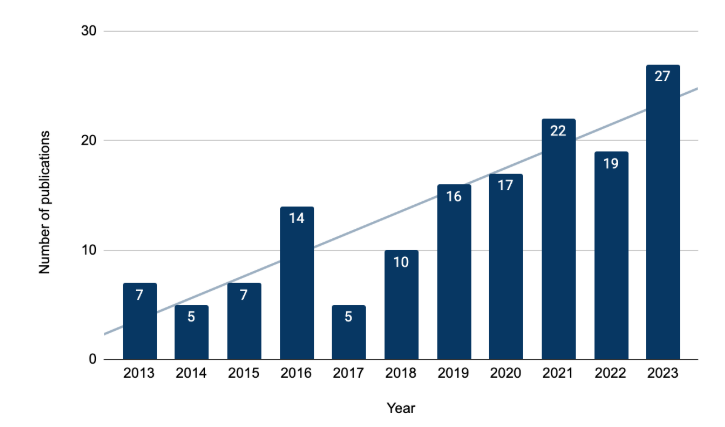
\includegraphics[width =\textwidth]{Imagens/Fig1.png}
\caption{Number of publications on digital local journalism by year.}
\label{fig-1}
\source{Authors’ work.}
\end{minipage}
\end{figure}

Interest in research on local digital journalism has grown over the period under analysis (2013–2023), with a visible increase in publications from 2017 onwards (Figure \ref{fig-1}). Within this sample, and unsurprisingly, the journal with the largest number of published articles fitting the criteria for this review is \emph{Digital Journalism} (27), followed by \emph{Journalism Practice} (17), \emph{Journalism Studies} (14), \emph{Journalism} (10), and \emph{Media and Communication} (4). The sample, however, is highly fragmented, comprising 61 different publications from very diverse regional scopes and contexts. Journals covering specific geographical areas are also significant within this sample, such as \emph{Nordicom Review} (10) and \emph{Media International Australia} (3), suggesting a relationship with the robust local news ecosystems found in the Nordic countries and Australia. The presence of books is also noteworthy, such as \emph{Local Journalism: Critical Perspectives on the Provincial Newspaper}, edited by \textcite{matthews2023}, which includes six chapters that suited the criteria for the systematic review review (\Cref{fig-2}).

%--- código da figura 2 ---%
\begin{figure}[htbp]
\centering
\begin{minipage}{0.70\textwidth}
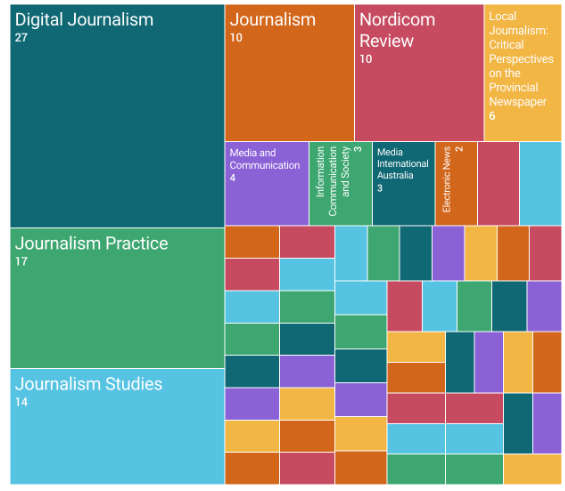
\includegraphics[width =\textwidth]{Imagens/Fig2.png}
\caption{Journals, books, or edited volumes with the highest number of published articles.}
\label{fig-2}
\source{Authors’ work.}
\end{minipage}
\end{figure}

Regarding authorship, 254 scholars were identified as authors or co-authors of these publications, representing fewer than two authors on average (M = 1.7) per publication. Considering the country of affiliation, around 30\% of them (78) are from universities and research centres in the United States. Scholars from the Global North are well represented, with the United Kingdom (40), Sweden (25), Norway (19), and Australia (15) making up most of the sample.

Most of the publications are journal articles (124); followed, in lesser numbers, by book chapters (14), books (5), and conference papers (6) (\Cref{fig-3}).

%--- código da figura 3 ---%
\begin{figure}[htbp]
\centering
\begin{minipage}{0.85\textwidth}
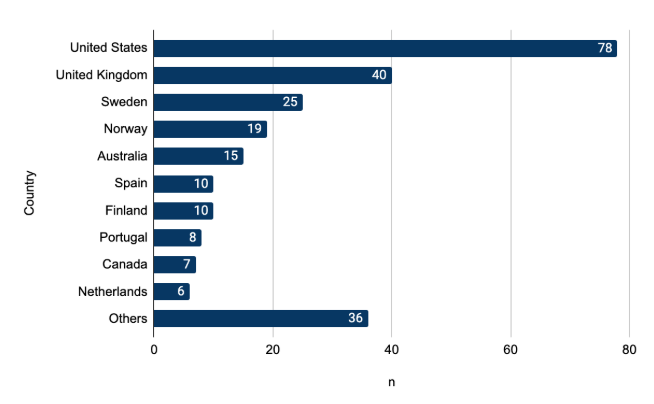
\includegraphics[width =\textwidth]{Imagens/Fig3.png}
\caption{Author affiliations by country.}
\label{fig-3}
\source{Authors’ work.}
\end{minipage}
\end{figure}

Most studies (129) focused on a single country, 16 analysed multiple countries, and 4 did not specify a geographical context. The United States was the most studied country regarding local digital journalism (42 publications), followed by the United Kingdom (21), Norway (17), Sweden (16), Australia (12), and Spain (7). Over the past ten years, research has concentrated on Western Europe, the Nordic countries, and the Anglophone Americas, a geographical distribution which was likely influenced by the criteria of this study which excluded non-English language publications and used the Scopus database. Some studies, however, do examine Asian and African contexts, such as Malaysia (3), Indonesia (2), Tanzania (1), Ethiopia (1), and South Africa (1).

The majority of the relevant studies are empirical in nature (141), with few theoretical approaches (8). There is a balance between qualitative (56) and quantitative (62) methods, with a slight predominance of the latter. Mixed methods are also common (23). The most frequently used qualitative methods include interviews, focus groups, observation, and case studies. Among quantitative approaches, surveys and content analysis stand out. Mixed methods combine surveys, interviews, focus groups, and observation (\Cref{fig-4}).

%--- código da figura 4 ---%
\begin{figure}[htbp]
\centering
\begin{minipage}{0.70\textwidth}
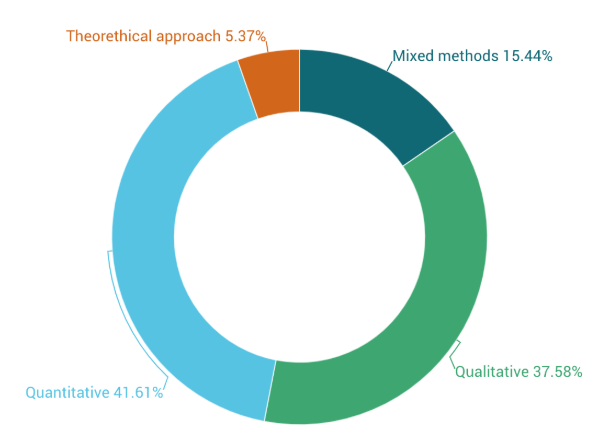
\includegraphics[width =\textwidth]{Imagens/Fig4.png}
\caption{Methodologies adopted in the analysed studies.}
\label{fig-4}
\source{Authors’ work.}
\end{minipage}
\end{figure}

\subsection{Content analysis}
The main themes under study in these publications can be grouped into six categories.

The first grouping (n=31) addresses journalistic practice and the roles of digital local media, including the social media usage, gaps in coverage, and characteristics of news outlets, and will be referred to as Journalistic Practice and Roles. The second (n=31) examines the ecosystem of digital local media, including mapping and other actors such as alternative and community journalism, and will be called Digital Local Media Landscape. The third (n=24) focuses on digital transformation and innovation, such as AI use, the role of algorithms, and the digitisation of journalism; it is labelled Digital Transformation. The fourth grouping (n=30), named Audience Research, concerns audience research, including social media interactions, citizen journalism, and news consumption. The fifth (n=24) covers Business Models, analysing the revenue streams and economic sustainability of digital local media. Finally, the grouping Civic Engagement (n=9) investigates the relationship between digital local media and civic and political participation.

Cross-referencing between the studied themes and countries did not reveal clear patterns, but some observations can be made: Studies related to civic engagement were highly relevant within the national sample of Australia (5); in Norway-focused studies, 7 of 17 publications examined the topic of business models; in Sweden and the United Kingdom, hyperlocal media stand out as a relevant subject, with 5 and 4 studies respectively; in the United States, research on journalistic practice and roles is more prevalent (12).

\subsubsection{Journalistic practice and roles in digital local media}

\subsubsubsection{Journalistic Practice}
With the digitisation of news production, distribution and consumption, local journalists must adapt their practices as well. The organisational culture of local newsrooms influences the way they respond to digital transformation \cite{ohara2023}. Many digital reporters still produce conventional stories based on traditional practices \cite{ryfe2016}. Digital local journalism in Europe as a whole suffers from superficiality and insufficient adaptation to online formats, but it could benefit from new ways of engaging audiences, such as transmedia storytelling \cite{rivasderoca2020}.

\subsubsubsection{Metrics and Their Effects}
As news increasingly relies on the digital space, local journalists and editors face a new type of pressure: traffic metrics, which can influence content selection and how stories are shared on social media, affecting newsroom practices and mobile journalism standards \cite{blanchettneheli2018, perreault2019}. To meet these pressures, many newsrooms pursue breaking news coverage and continuous updates, a practice which local journalists see as potentially harmful but necessary to maintain audience credibility \cite{usher2018}. In this context, digital local journalists face high workloads, tight deadlines, and limited labour protections \cite{higginsdobney2021}. This reliance on traffic metrics, which prioritise superficiality and click volume, poses a significant risk of drift in journalism, diverting focus from in-depth investigation and core ethical responsibilities.

Audience data also influence gatekeeping on news websites and shape future coverage \cite{blanchett2021}. Other metrics, such as audience awareness and public impact, are used by local journalists to evaluate their civic contributions \cite{powers2018}.

\subsubsubsection{Social Media Use by Journalists}
Widespread social media use has highlighted its potential as a source and dissemination tool for local journalists, who use it to identify trends and engage with audiences, a practice which was only accelerated by the Covid-19 pandemic \cite{zhang2022}. Perceiving social media as a credible information source is positively associated with its use in news production \cite{zhang2020}. Social media enables journalists to integrate more hyperlocal and data-driven narratives, employing innovative elements such as affective storytelling \cite{chen2023}.

Local journalists construct their online personas under the influence of audiences and platform affordances, combining professional and personal aspects in their identity \cite{baftiu2023}. Online, they engage in information flows among elites \cite{habel2018}, while also being compelled to use social media as an accountability tool \cite{slavtchevapetkova2016}. The likelihood of journalists developing an online persona is guided by institutional readiness \cite{hamzah2020}.

However, digital presence brings challenges, such as the spread of fake news, which affects journalistic work. In countries like Indonesia, journalists believe organisational policies influence how they handle misinformation, leading them to rely on official sources to debunk false news \cite{kwanda2020}.

\subsubsubsection{Journalistic Roles}
Despite pressures, journalists working for digital local media continue producing journalism that serves community needs, with local focus becoming increasingly defining \cite{sjovaag2015}. Local journalism continues to reflect traditional news values while embracing diverse forms of journalism \cite{jenkins2020b}, fulfilling informational, commercial, and community cohesion roles \cite{matthews2023}. Role interpretations vary across outlets, with regional TV, radio, online, and print journalists holding different perceptions \cite{fisher2022}.

In digital journalism startups, journalists adopt more relational and meaningful knowledge production practices, also acting as community advocates \cite{anderson2023}. Altruistic roles, such as service provision, are particularly important in these startups, especially in news deserts \cite{finneman2022}.

\subsubsection{Digital local media landscape}
\subsubsubsection{Local media landscape}
Even within newspapers’ digital transition, diminishing their role in local media ecosystems that develop unevenly and with uncertain futures \cite{nielsen2015}, geography remains relevant towards understanding the concept of ``local" in digital journalism. This includes not only territorial boundaries but also the absence of limits and the opening of the social space in which newspapers operate, what \textcite{hess2013} calls ``geo-social" news.

Research on local news information flows has been explored through various methods, including mapping, which identifies ``news deserts" where there is little or no journalistic coverage.

In African countries, online news deserts are found in regions or countries rarely covered by online media \cite{madridmorales2023}. In Europe, for instance, studies in Spain show depopulation as a crucial factor in local media loss. \textcite{negreira-rey2023} identified ``news deserts" in Spain, while \textcite{negredo2023} mapped digital media to analyse characteristics such as their platform, geographical scope, and language. In the UK, \textcite{bisiani2023} revealed deficiencies in local media databases, generating data for future research on local news availability and gaps. Understanding these news gaps is crucial as the absence of robust local news provision can have significant consequences for local civic information infrastructure, particularly during emergencies, which became clear during the Covid-19 pandemic \cite{battocchio2023}.

In the United States, there has been a proliferation of websites disguising their nature as political propaganda vehicles under the guise of  local media outlets, copying content and exploiting political controversies and emotions to generate engagement \cite{karell2022}.

\subsubsubsection{Hyperlocal Media}
Research on hyperlocal journalism, community-led news operations, gains traction in the context of loss of relevance of local newspapers, matched by an increase in the importance of online community news. This type of research aims to understand the impact of local newspaper disappearance on the communities that are seeing their papers replaced by digital news providers \cite{harte2018}.

In this context of newspaper closures, hyperlocal initiatives are often expected to fill the remaining gap. In Sweden, however, most hyperlocal projects are in urban and metropolitan areas, and coexist with traditional media, leaving other regions that are losing their newspapers as news deserts \cite{jangdal2019, nygren2018}. In Norway, \textcite{halvorsen2019} observed that online hyperlocal outlets avoid competing with traditional media but are present in different types of municipalities.

European research indicates that hyperlocal media projects are driven by the desire to engage people in community-building. These outlets provide local news but face human and financial resource limitations, hindering the search for sustainable business models \cite{hujanen2019, negreira-rey2022, tenor2019}. Only a small proportion of these projects generate sufficient revenue to operate professionally \cite{halvorsen2019}.

These outlets range from fully staffed operations to individually run sites, but they share common challenges such as performance and revenue \cite{vankerkhoven2014}. Depending on the local context, hyperlocals may act more collaboratively than competitively with traditional media \cite{dovbysh2021}.

Their importance is evident: \textcite{hujanen2021} investigated the civic roles of hyperlocal media professionals in Sweden, Finland, and Russia, showing them as information providers, community builders, and civic mediators, reflecting media and political contexts. Role conceptions centred on social cohesion have also been investigated in Australia \cite{barnes2022}.

Civic roles may vary according to hyperlocal professionalisation and business model (for-profit or nonprofit) \cite{tenor2018}. Research in the UK concluded that hyperlocal projects play a key role in providing information on community activities, amplifying citizens’ voices \cite{williams2015}, fostering proximity to audiences \cite{harte2017}, while negotiating different discourses on their value \cite{harte2023}.

\subsubsubsection{Citizen Journalism and Audience Participation}
Audience participation is an essential feature of digital local journalism. Research on citizen journalism focuses on participation and mobilisation, highlighting its democratic and revitalising role \cite{harcap2016, blom2014}. Local newsrooms promote citizen engagement, creating strong community ties through journalism. In this context, ``participation" takes on several meanings: commodification, co-production, and democratic involvement that helps to shape local journalistic identity \cite{carlsson2016}.

Social media amplify these trends, increasing audience involvement in the dissemination of local news, but challenges emerge concerning verification and the quality of citizen-generated content. Research has also explored audience participation in digital platforms, where the community helps to alleviate staff shortages in local newsrooms \cite{cook2021}.

\subsubsection{Digital transformation and its impacts on local journalism}
\paragraph{Digital transformation and the influence of digital technologies in newsrooms}
As news migrates from print to online formats, newspapers face challenges in adapting to new economic, social, and technological realities, which  precipitate changes in news production, audience interaction \cite{anderson2013}, and innovations such as the impact of computational journalism \cite{young2015}.

By adopting a ``digital first" model, regional newspapers in the United Kingdom began prioritising online news, adjusting to audience preferences \cite{clark2023}. Digital culture accelerates the rhythms of content production, transforming news dissemination into a high-speed process \cite{hagen2022, hradziushka2020}. This digitisation process has particularly hindered smaller newspapers, which struggle with digital distribution, changes in working practices, and the adoption of new tools \cite{ali2019}. During the Covid-19 pandemic, digital transformation was central in some regions \cite{gurkan2023}, while in others local journalists had a limited understanding of the importance of their online presence \cite{ivask2024}.

In thies digital shift, many local journalists challenged the traditional structures of the organisations they work for, innovating by restructuring practices and products to attract digital audiences \cite{jenkins2021}. However, despite recognising the importance of technology for their continued viability, many face a lack of technical skills, such as search engine optimisation and digital content creation \cite{esa2022}.

In Portugal, the integration of digital technologies into the routines of local journalists has been limited: although these tools are widely used to gather news and contact sources, few journalists employ them to engage with the community and incorporate citizen-generated content \cite{jeronimo2022}.

\paragraph{Innovation and technological adaptation}
Although innovation and artificial intelligence are emerging themes in journalism research, they appear in only a few articles within this sample, more closely linked to innovation strategies and their adoption in organisations.

Innovation strategies, from multimedia and AI usage to business model change, shape how media outlets deal with constraints and their need for public support \cite{wilczek2021}. Business models also have an impact on innovation; media outlets owned by conglomerates benefit from shared resources such as audience analytics \cite{puijk2021}.

Emerging research topics in this field include Journalism of Things (JoT) and innovation practices in local journalism \cite{hamm2022}, and the adaptation of AI and algorithms for use in local newsrooms \cite{dralega2023}. It is crucial to explore how automation may redefine journalistic practices, from news content generation to curation and distribution, and the ethical and labour implications for local journalists.

\paragraph{Platformisation}
Platforms, especially social media, play an increasingly important role in local media ecologies. The influence of social media, search engines, and recommendation services compels traditional media outlets to create content for popular platforms such as Instagram and TikTok, where the boundaries between news and entertainment are blurred and audience engagement becomes the primary metric \cite{hradziushka2022}. This scenario raises critical questions about control of information and editorial freedom, as platforms, with their own economic incentives and algorithms, can end up steering editorial decisions, limiting content diversity and, consequently, the role of local journalism in democracy \cite{fuchs2014social}.

Although in some European contexts such as Sweden, audiences use Facebook for local news more than they use online local newspapers, the latter are still regarded as more important sources, despite declining readership. Online newspapers, public service outlets, and hyperlocals coexist in Facebook’s public sphere \cite{nygren2019}. Yet the economic incentives of digital platforms can divert editorial decisions away from local news, since Facebook favours certain types of content over others \cite{toff2021}. \textcite{firmstone2021} also observed that using social media to distribute content may undermine journalists’ editorial authority, as audiences determine the agenda and digital practices weaken the local relevance of news by privileging viral or breaking stories.

Platformisation also affects journalists' work and news distribution. Although platform presence is seen as essential, local media professionals fear that the public may not be able to distinguish their organisations’ content from other material circulating online \cite{morais2023}. This also affects the visibility of news and the reach of online media outlets focused on specific communities, due to the semantic mechanisms underpinning platforms and distributing news \cite{ivancsics2023}. These mechanisms not only filter content but also shape how messages are encoded and decoded, influencing meaning-making and how audiences interpret the news.

\subsubsection{Audience research}
\paragraph{Audience preferences for news consumption}
Local journalism is closely tied to its audiences, due to the proximity of information and shared cultural values. The study of audience interactions and news consumption preferences is crucial in the field of digital local news, as are aspects related to language and format, particularly visual and interactive elements, which shape preferences.

Attitudes towards online news consumption have been analysed in various geographical contexts. In Portugal, despite uncertainties, local audiences still prefer traditional formats such as print and radio for news consumption, although they consider websites and Facebook to be the most dynamic digital spaces for seeking information \cite{ribeiro2021}. In Australia, \textcite{hess2023} observed that, in addition to a continued desire for print media, there is a strong attachment to the local identity behind content and its production. In Norway, research revealed that the greatest audience overlap is between online local newspapers and Facebook, with offline media outlets being more valued and seen as democratic resources for local public life than online ones are \cite{olsen2020}. However, social media presence does not always result in greater audience engagement \cite{solvoll2020}.

Regarding online news, local audiences perceive it as personally relevant or interesting information, as content produced by local media brands, and as community engagement \cite{guyas2019}. The practices of digital local news audiences to stay updated on local events can be understood from three perspectives: an  individual responsibility of staying informed and reliance on the “news-finds-me” effect, a lack of involvement with the production and dissemination of journalism, and the continuing importance of interpersonal networks as sources of local information \cite{mccollough2017}.

\paragraph{Interaction between journalists and audience}
The emergence of the Internet and social media created a more participatory media ecology, allowing audiences to interact with journalists and media outlets more quickly, cheaply, and accessibly than previous technologies allowed. These interactions have been widely studied in the context of digital local journalism.

One of the main forms of direct interaction was the use of news comments, a public space shaped by the media outlet but appropriated by audiences. This practice was more extensively studied in the early years of the interval under analysis. In Sweden, \textcite{almgren2015} observed that while media outlets prefer to allow comments on lighter news, such as sport and entertainment, the public prefers to comment on more impactful topics, such as politics and health. As more news sites adopted interactive features, comments grew exponentially, creating challenges for journalists dealing with user-generated content. While acknowledging the democratic function of comments, journalists also worry about brand-related risks and the need to allocate significant resources to managing this kind of audience interaction \cite{canter2013}. In Sweden, local newspapers have a greater tendency to allow comments on their online articles than national media outlets \cite{almgren2016}.

As the years passed and social media gained greater prominence, research shifted to these platforms to understand audiences’ practices and attitudes towards the changing relationship with journalists. In comments on social media news links, particularly on Facebook, incivility became a key topic of study \cite{kim2023}. Audiences on these platforms also act as secondary gatekeepers, selecting news items to share within their networks. Facebook, for example, has considerable influence in news dissemination, with local audiences preferring to share lighter stories, often from internal sources, such as neighbourhood changes or healthcare \cite{almgren2017}. Engagement with news has also been studied on messaging apps such as Telegram, where emotional content and videos were found to generate greater interaction \cite{hradziushka2023}.

\subsubsection{Business models}

\paragraph{Revenue mix and business strategies}

Research on business models for local news addresses the challenges posed by economic crises in traditional media, while large technology companies such as Google and Facebook dominate audiences’ online time and reap the profits \cite{hindman2018}. Many local media outlets continue to prioritise their print products, even in the face of falling advertising and subscriptions revenue, while their business strategies, still rooted in the analogue era, now attempt to adapt to the digital world \cite{jenkins2020a,cestino2023}. Paid content is emerging as a relevant approach \cite{jenkins2023}.

In Norway, the consolidation of economic groups in the digitisation process has been analysed in terms of pluralism and organisational suitability. The lack of independence in digital media ownership has led to consolidation as a solution for technological resources and economies of scale, but differentiation strategies remain essential for local newspapers, even with reduced staff \cite{sjovaag2014,sjovaag2021}.

In Spain, advertising remains the most popular source of revenue for digital news operations, with local and regional news outlets displaying very low diversification of revenue streams and a less innovative mix of income compared to their national counterparts \cite{varamiguel2021}.

Studies have also explored the performance of digital local news start-ups, showing that those with lower revenue publish fewer stories than those with higher revenue \cite{chadha2019}. Ownership, funding mechanisms, and organisational mission influence the type of content that digital local media outlets produce \cite{harlow2021}.

The role of paywalls is another central theme in research on digital local media. Findings indicate that the most valuable journalistic content is placed behind paywalls, while high-traffic news stories remain open to non-subscribers \cite{sjovaag2016,kvalheim2013}. Although paywalls offer a new revenue stream, they also reduce the number of views and visitors, jeopardising the civic function of local news \cite{olsen-etal2020}. Paywall strategies vary: one focuses on existing customers with differentiated products, while another targets the advertising market by optimising user data \cite{olsen2018}.

\paragraph{Paying for news}
The willingness to pay for online local news is influenced by factors such as local coverage, community ties, age, gender, and past news consumption habits \cite{goyanes2015}, and trust in local journalism and perceptions of content quality also play a crucial role in readers’ subscription decisions \cite{park2022}.

At the same time, structural and relational obstacles, as well as the regularity of reading habits and the amount of local content that is published, may reduce willingness to subscribe or lead to subscription cancellations \cite{ross2021, kim2021}. Digital subscribers pay less than print ones and do not contribute very significantly to newspapers’ total revenue \cite{chyi2020}.

\subsubsection{Civic engagement}
Local journalism has proved essential in promoting civic engagement and a sense of belonging. Research indicates that, in addition to being rooted to a specific geography, local journalism harbours a deep understanding of places and community dynamics \cite{hess2016}.

Digital technologies may facilitate community ties and civic engagement, and they may (or may not) strengthen social cohesion and community identity, a multifaceted reality that requires further exploration. On the one hand, digital local media position themselves as ``guardians" of the civic virtue of the communities they serve \cite{hess2016}. The use of local digital newspapers as a source of information leads to greater participation in community activities \cite{thompson2021}. On the other hand, community groups, especially on Facebook, create other forms of civic engagement and are becoming a preferred news source, often surpassing local media \cite{carlsson2016}.

The relationship between digital local media and democracy has also been studied in the context of elections in the United States. Although the use of digital media has not been a consistent predictor of electoral participation, the use of traditional media has \cite{min2022}. However, there is a null long-term effect of exposure to local news sites on political participation, knowledge, and affective and attitudinal polarisation, which is attributed to the low use of news sites \cite{cronin2023}.

\section{Discussion}
In this article, we propose a review of a decade of research on digital local journalism (2013–2023). The findings reveal that there has been an increased academic focus on the impacts of digitisation on journalistic practices, media landscapes, and local audience engagement. Both over time publication growth and the concentration of articles in journals such as \emph{Digital Journalism} confirms there is a growing interest and consolidation of the topic within digital journalism studies, in line with the field’s evolution towards a focus on technology and platforms.

 Regarding RQ1, the main themes that can be identified include changes in journalistic roles, the influence of digital platforms, audience interactivity, and the development of sustainable business models. These themes directly reflect the challenges of journalists’ continuous adaptation to new digital demands, the need for innovation in the face of the crisis of traditional business models, and the increasing complexity of relations with audiences in fragmented online environments. These findings align with trends observed in recent literature reviews, such as the discussion on business models, platforms, ``news deserts", proximity in journalistic practices, and audience interaction.

 Research across 2013–2023 reflects the challenges faced by local journalists in adapting to the digital world. The acceleration of content production, alongside diminishing human resources, resulted in increased superficiality and a lack of adaptation to novel online formats. Traffic metrics influenced newsroom practices, shaping coverage and being used to assess civic contributions. Furthermore, journalists struggle with a lack of technical skills.

 The organisation of journalistic work was also impacted. The relationship between local journalism, journalists, and social media stands out as a central theme. Local journalists use social media to obtain and verify sources, increasingly relying on these platforms as their use grows, and incorporating hyperlocal and affective narratives into coverage. However, digital platforms affect the visibility of news and can steer editorial decisions towards a strategy of higher social media or platform reach, undermining the public interest of local news coverage. This dynamic raises serious concerns about the editorial independence of local media outlets and the upholding of quality standards, such as fact-checking and journalistic ethical principles, which are essential for local media’s democratic role. Research also highlights the overlap of audiences between online local newspapers and Facebook.

Regarding RQ2, studies reveal a predominant focus on the Global North, with the United States being the most studied country, followed by the United Kingdom. Almost half of the sample (45\%) was concentrated in four influential journals published by UK and US academic publishers. The gap in geographical representation highlights the need for more studies on digital local journalism in the Global South, particularly in regions such as Latin America, parts of Asia, and Africa, where the dynamics of technology access, business models, and sociopolitical contexts vary significantly and offer unique perspectives. This pattern reflects the geographical representation of the most influential databases and languages in Communication Studies.

\section{Conclusions}
Throughout this systematic review, covering a decade of research on digital local journalism (2013–2023), it was possible to observe the remarkable growth of academic interest in the subject, reflected in the increase in publications from 2017 onwards and the dedication of influential journals such as \emph{Digital Journalism}. The findings reveal six predominant research clusters, with particular emphasis on transformations in journalistic practices, the impact of digital platforms, and the pursuit of sustainable business models, demonstrating an evolution of research in line with broader trends in digital journalism. However, the concentration of studies in the Global North underscores the need for a more diversified perspective.

Digital local media -- whether hyperlocal projects or extensions of traditional media outlets -- continue to play a crucial role in disseminating information and fostering social cohesion in communities, encouraging participation in local activities and groups, despite persistent gaps in news coverage and sustainability challenges.

Future research should explore the role of local journalism in building trust and stimulating community engagement, examining how digitisation and platformisation can both consolidate and fragment community identity and social cohesion, particularly by exploring contexts beyond those already studied. Furthermore, it is essential to investigate the impact of algorithmic gatekeeping and the dependence on digital platforms for visibility and sustainability in local journalism. The relationship between proximity and reliance on these platforms for funding, content gathering, and distribution deserves greater attention, as is already the case in journalism studies more broadly.

Other emerging themes, such as changing patterns of news consumption, the active search for local information, incidental exposure, and the growing avoidance of news, should be analysed in local contexts to better understand the challenges and opportunities of digital journalism.


\section{Funding}
The authors would like to thank the \emph{Fundação para a Ciência e a Tecnologia (FCT)} for the fun\-ding of MediaTrust.Lab (\url{http://doi.org/10.54499/PTDC/COM-JOR/3866/2020}), the project that led to this study; Pedro Jerónimo’s  contract  (\url{https://doi.org/10.54499/CEECINST/00016/2021/CP2828/CT0004}); Luísa Torre’s doctoral scholarship (2023.05397.BD) and LabCom  (\url{http://doi.org/10.54499/UIDB/00661/2020}), the centre where the authors conduct their research.


\printbibliography\label{sec-bib}
% if the text is not in Portuguese, it might be necessary to use the code below instead to print the correct ABNT abbreviations [s.n.], [s.l.]
%\begin{portuguese}
%\printbibliography[title={Bibliography}]
%\end{portuguese}

%full list: conceptualization,datacuration,formalanalysis,funding,investigation,methodology,projadm,resources,software,supervision,validation,visualization,writing,review
\begin{contributors}[sec-contributors]
\authorcontribution{Pedro Jerónimo}[conceptualization,funding,methodology,projadm,supervision,validation,writing,review]
\authorcontribution{Luísa Torre}[datacuration,formalanalysis,investigation,methodology,validation,visualization,writing]
\end{contributors}



\end{document}

